% Options for packages loaded elsewhere
\PassOptionsToPackage{unicode}{hyperref}
\PassOptionsToPackage{hyphens}{url}
%
\documentclass[
]{article}
\usepackage{amsmath,amssymb}
\usepackage{lmodern}
\usepackage{iftex}
\ifPDFTeX
  \usepackage[T1]{fontenc}
  \usepackage[utf8]{inputenc}
  \usepackage{textcomp} % provide euro and other symbols
\else % if luatex or xetex
  \usepackage{unicode-math}
  \defaultfontfeatures{Scale=MatchLowercase}
  \defaultfontfeatures[\rmfamily]{Ligatures=TeX,Scale=1}
\fi
% Use upquote if available, for straight quotes in verbatim environments
\IfFileExists{upquote.sty}{\usepackage{upquote}}{}
\IfFileExists{microtype.sty}{% use microtype if available
  \usepackage[]{microtype}
  \UseMicrotypeSet[protrusion]{basicmath} % disable protrusion for tt fonts
}{}
\makeatletter
\@ifundefined{KOMAClassName}{% if non-KOMA class
  \IfFileExists{parskip.sty}{%
    \usepackage{parskip}
  }{% else
    \setlength{\parindent}{0pt}
    \setlength{\parskip}{6pt plus 2pt minus 1pt}}
}{% if KOMA class
  \KOMAoptions{parskip=half}}
\makeatother
\usepackage{xcolor}
\usepackage[margin=1in]{geometry}
\usepackage{graphicx}
\makeatletter
\def\maxwidth{\ifdim\Gin@nat@width>\linewidth\linewidth\else\Gin@nat@width\fi}
\def\maxheight{\ifdim\Gin@nat@height>\textheight\textheight\else\Gin@nat@height\fi}
\makeatother
% Scale images if necessary, so that they will not overflow the page
% margins by default, and it is still possible to overwrite the defaults
% using explicit options in \includegraphics[width, height, ...]{}
\setkeys{Gin}{width=\maxwidth,height=\maxheight,keepaspectratio}
% Set default figure placement to htbp
\makeatletter
\def\fps@figure{htbp}
\makeatother
\setlength{\emergencystretch}{3em} % prevent overfull lines
\providecommand{\tightlist}{%
  \setlength{\itemsep}{0pt}\setlength{\parskip}{0pt}}
\setcounter{secnumdepth}{-\maxdimen} % remove section numbering
\ifLuaTeX
  \usepackage{selnolig}  % disable illegal ligatures
\fi
\IfFileExists{bookmark.sty}{\usepackage{bookmark}}{\usepackage{hyperref}}
\IfFileExists{xurl.sty}{\usepackage{xurl}}{} % add URL line breaks if available
\urlstyle{same} % disable monospaced font for URLs
\hypersetup{
  pdftitle={Trabalho Metodos de Regressao},
  pdfauthor={Victor Telles; Felipe Carmo; Leandro Barros},
  hidelinks,
  pdfcreator={LaTeX via pandoc}}

\title{Trabalho Metodos de Regressao}
\author{Victor Telles; Felipe Carmo; Leandro Barros}
\date{2023-10-05}

\begin{document}
\maketitle

\hypertarget{resumo}{%
\section{Resumo}\label{resumo}}

O comércio eletrônico no Brasil experimentou um crescimento
significativo nas últimas décadas, tornando-se uma parte essencial do
cenário de varejo do país. Com uma população numericamente grande e uma
economia em crescimento, o Brasil viu um aumento notável nas transações
de comércio eletrônico. Milhões de brasileiros agora preferem fazer
compras online, aproveitando a conveniência de encontrar uma ampla
variedade de produtos e serviços sem sair de casa. Plataformas de
comércio eletrônico e marketplaces desempenham um papel fundamental
nesse ecossistema, conectando consumidores a uma vasta gama de
vendedores e produtos.

Apesar dos desafios logísticos e de infraestrutura, o comércio
eletrônico no Brasil continua a atrair investimentos e inovações. A base
de dados ``Brazilian E-Commerce Public Dataset by Olist'' oferece
insights valiosos sobre as transações e comportamento dos consumidores
nesse mercado em constante evolução, permitindo análises detalhadas e
tomada de decisões informadas.

A fim de entender melhor o comportamento do comércio eletrônico, o
trabalho contempla análise com métodos estatísticos explicados na
disciplina Regressão Linear, tais como análise descritiva de dados,
análise de multicolineareida, entendimentos de valores influentes,
verificação de parâmetros da tabela ANOVA, aplicação de teste de
hipoteses como Kolmogorov-Smirnov, Breush-Pagan e seleção de modelos, na
base de dados da Olist a fim de entender como se relaciona o preço do
frete em decorrência de variáveis como tamanho e peso do produto
entregue, distância entre compradores e vendedores, data da entrega,
dentre outras.

\hypertarget{introduuxe7uxe3o}{%
\section{Introdução}\label{introduuxe7uxe3o}}

A análise preditiva desempenha um papel crucial na gestão eficaz das
operações de comércio eletrônico, especialmente no que diz respeito ao
cálculo de frete. A fim de entender melhor o comércio eletrônico
brasileiro, foi encontrada a base de dados ``Brazilian E-Commerce Public
Dataset by Olist'' que permite explorar e entender as complexas
variáveis que influenciam o custo de frete no contexto do comércio
eletrônico no Brasil.

Sendo o frete é um dos principais fatores que impactam a experiência do
cliente e os custos operacionais das empresas de comércio eletrônico.
Torna-se aprazível buscar calcular da maneira objetiva o custo do frete
envolvendo várias variáveis interconectadas, como a quantidade de
produtos entregues, o valor do pedido do produto, o volume do pedido, a
distância da entrega, a quantidade de dias para entregar o produto e o
peso do produto.

Nesse cenário complexo, a regressão linear surge como uma ferramenta
para prever os custos de frete com base nessas variáveis. Através da
análise preditiva, podemos tentar explorar as relações entre essas
variáveis e os custos de frete, identificando tendências e padrões que
podem ajudar a tomada de decisões mais clarividentes.

Através da análise de dados da base: ``Brazilian E-Commerce Public
Dataset by Olist'', é possível entender e justificar a aplicação da
análise preditiva por regressão linear a fim de estimar os custos de
frete no contexto do comércio eletrônico brasileiro. Com essas
estimativas pretende-se fornecer insights valiosos que buscam otimizar
processos logísticos, melhorando a satisfação do cliente para que haja a
tomada de decisões estratégicas baseadas em dados sólidos.

Durante o curso deste trabalho, iremos analisar cuidadosamente as
variáveis disponíveis na base de dados, construir modelos de regressão
linear e avaliar sua eficácia na previsão dos custos de frete. Além
disso, discutiremos como essa análise pode contribuir para a redução de
custos operacionais e a otimização das operações de entrega.

\hypertarget{materiais-e-muxe9todos}{%
\section{Materiais e Métodos}\label{materiais-e-muxe9todos}}

\hypertarget{desenho-do-estudo}{%
\subsection{Desenho do Estudo}\label{desenho-do-estudo}}

Neste capítulo, detalharemos os materiais e métodos utilizados para
desenvolver e analisar nosso modelo de regressão linear múltipla. O
objetivo deste estudo é investigar as variáveis que influenciam o valor
do frete a ser pago em um e-commerce brasileiro, considerando dados de
pedidos realizados entre 2016 e 2018, com uma amostra de cerca de
100.000 pedidos.

\hypertarget{coleta-de-dados}{%
\subsection{Coleta de Dados}\label{coleta-de-dados}}

\hypertarget{fonte-de-dados}{%
\subsubsection{Fonte de Dados}\label{fonte-de-dados}}

Os dados para este estudo foram obtidos do banco de dados de um market
place brasileiro, que registra informações detalhadas sobre pedidos
realizados entre 2016 e 2018, e disponibilizado na plataforma kaggle
para fins de análise pública, através do
link:\url{https://www.kaggle.com/datasets/olistbr/brazilian-ecommerce}.
A fonte de dados foi selecionada devido à sua relevância, para os
autores, por se tratar de um problema real, próximo da realidade
profissional vivenciadas por eles, devido ao tamanho da base de dados,
além de relevante para comunidade ter o entendimento dos fatores que
afetam o valor do frete em transações online e uma projeção do quanto
pagaria.

\begin{figure}
\centering
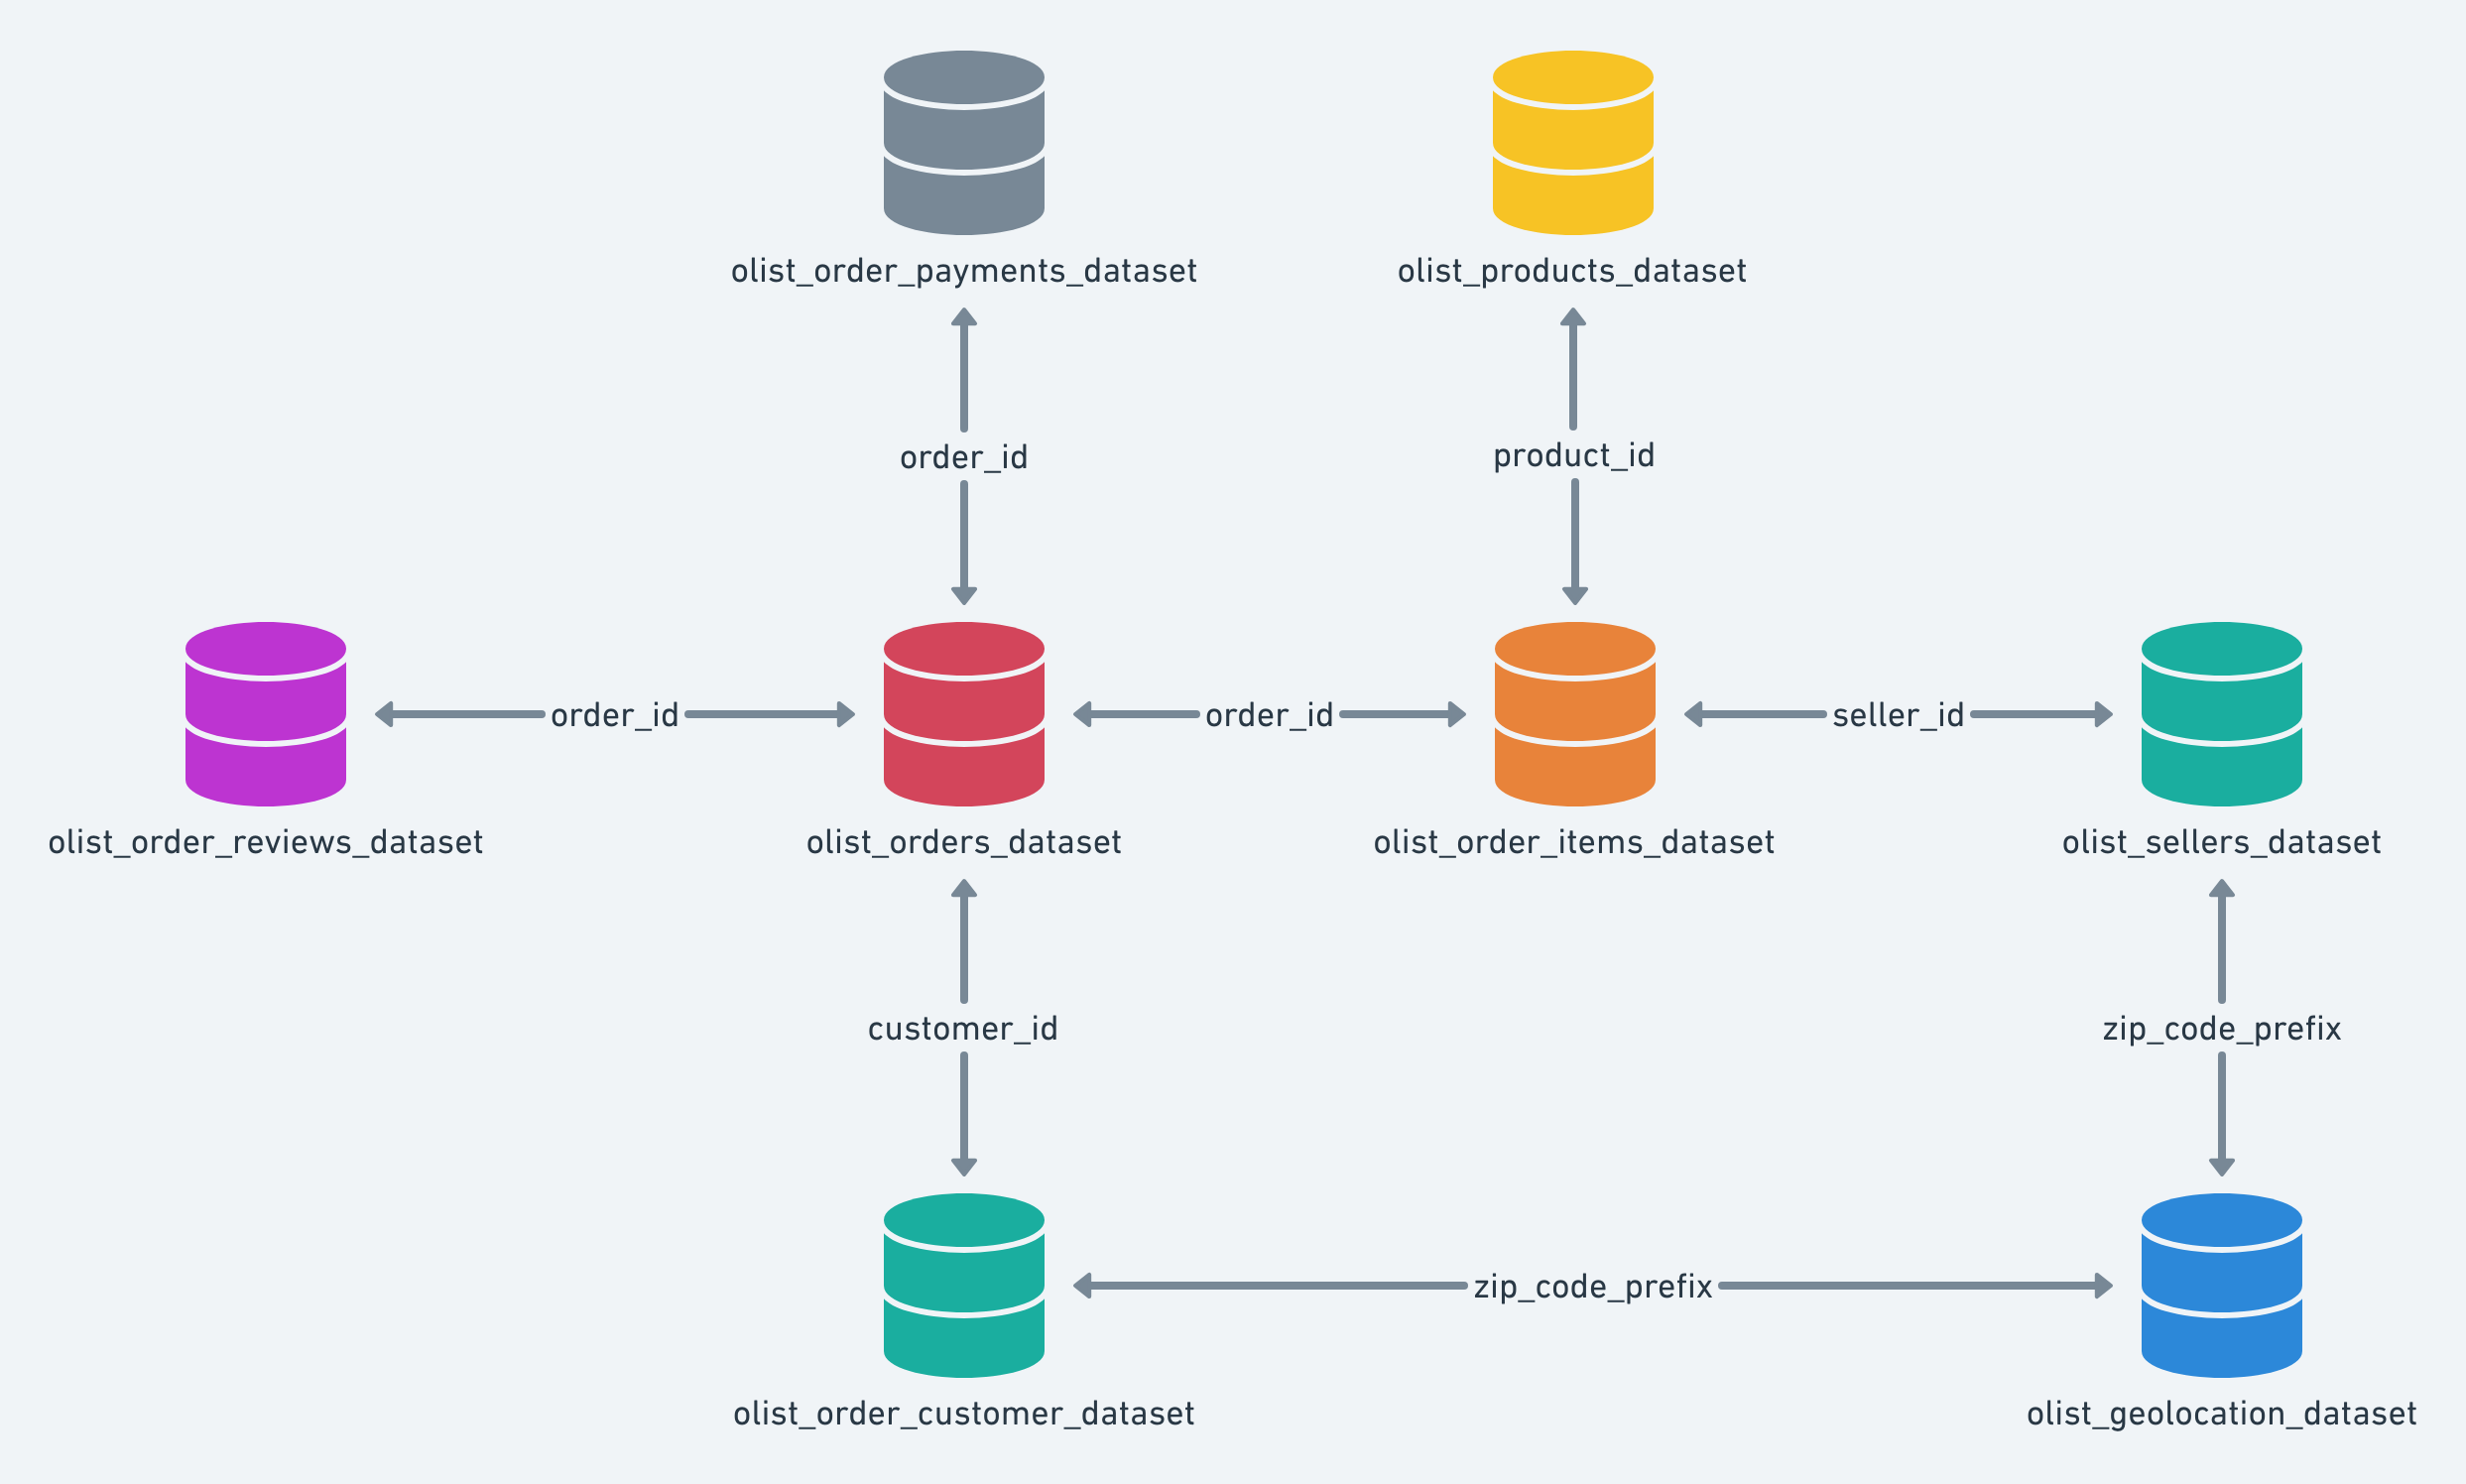
\includegraphics{/Users/victortelles/Documents/Coursera/Especializacao - UFMG/04 - Modelagem de relacoes usando Regressao Linear/Trabalho/HRhd2Y0.png}
\caption{Figura 1: Esquemático relacional entre as bases de dados
utilizada. Disponível em:
\url{https://www.kaggle.com/datasets/olistbr/brazilian-ecommerce}}
\end{figure}

Descrição das bases de dados quem compõem o sistema da Figura 1:

\begin{itemize}
\tightlist
\item
  Pedidos (Orders): Informações sobre os pedidos feitos pelos clientes,
  incluindo data do pedido, identificação do pedido, status do pedido e
  identificação do cliente.
\item
  Itens de Pedido (Order Items): Detalhes sobre os itens individuais
  dentro de cada pedido, incluindo identificação do produto, preço,
  quantidade, e o valor total do item.
\item
  Produtos (Products): Informações sobre os produtos disponíveis para
  compra, incluindo nome do produto, categoria, preço e peso.
\item
  Clientes (Customers): Dados sobre os clientes que fizeram os pedidos,
  incluindo identificação do cliente, nome, cidade e estado.
\item
  Pagamentos (Payments): Detalhes sobre os pagamentos associados a cada
  pedido, incluindo método de pagamento, valor do pagamento e
  parcelamento, quando aplicável.
\item
  Vendedores (Sellers): Informações sobre os vendedores que forneceram
  os produtos, incluindo identificação do vendedor, nome, cidade e
  estado.
\item
  Avaliações (Reviews): Avaliações e classificações dadas pelos clientes
  aos produtos e ao serviço de entrega.
\item
  Geolocalização (Geolocation): Dados de geolocalização que relacionam
  códigos postais às regiões geográficas no Brasil.
\item
  Categorias de Produtos (Product Categories): Informações sobre as
  categorias às quais os produtos pertencem.
\end{itemize}

\hypertarget{amostragem}{%
\subsubsection{Amostragem}\label{amostragem}}

Foram utilizados todos os pedidos observados no banco de dados, desde
que tivesse sido ``entregue'', não possuisse variáveis nulas ao fazer as
combinações com as demais bases de dados, o peso do produto fosse maior
que zero, o volume do produto fosse maior que zero, a distância entre
vendedor e comprador fosse maior que zero e menor que a maior distancia
em linha reta do Brasil (4.394 km), pedido que cujo pagamento não
tivesse utilização de voucher. Com aplicação de todas estas restrições
foram obtidas 94.995 observações para compor o modelo.

\hypertarget{variuxe1veis}{%
\subsubsection{Variáveis}\label{variuxe1veis}}

As variáveis utilizadas neste estudo incluem:

Variável Dependente (Y): Valor do Frete - Esta é a variável que
pretendemos prever com base nas variáveis independentes.

Variáveis Independentes (X1, X2, X3, \ldots): As variáveis explicativas
incluem: - Caracteristicas do Pedido (por exemplo, valor total,
quantidade de itens)

\begin{itemize}
\item
  Características do Produto (Peso, volume).
\item
  Características do Cliente (por exemplo, cep, latitude e longitude).
\item
  Características do Vendedor (por exemplo, cidade, localização).
\item
  Distância entre CEPs do Cliente e do Vendedor.
\item
  Características de tempo (por exemplo, dia da semana da compra, época
  do ano).
\end{itemize}

\hypertarget{modelagem-estatuxedstica}{%
\subsection{Modelagem Estatística}\label{modelagem-estatuxedstica}}

\hypertarget{modelo-de-regressuxe3o-linear-muxfaltipla}{%
\subsubsection{Modelo de Regressão Linear
Múltipla}\label{modelo-de-regressuxe3o-linear-muxfaltipla}}

Para realizar a análise, utilizamos um modelo de regressão linear
múltipla. buscando encontrar uma equação para o modelo como a seguinte:
Frete = β0 + β1X1 + β2X2 + \ldots{} + βnXn + ε

Onde:

Frete é o valor do frete.

\begin{itemize}
\tightlist
\item
  X1 ,X2 ,\ldots,Xn representam as variáveis explicativas mencionadas
  anteriormente.
\item
  β0 é o intercepto.
\item
  β1 ,β2 ,\ldots,βn são os coeficientes de regressão das variáveis
  independentes.
\item
  ε é o termo de erro
\end{itemize}

Neste estudo, foi aplicado o método stepwise para seleção de variáveis
no modelo. O método stepwise nos permitiu avaliar e selecionar
automaticamente as variáveis independentes mais relevantes com base em
critérios estatísticos, incluindo o critério BIC (Bayesian Information
Criterion). O critério BIC é particularmente útil, pois considera tanto
a qualidade de ajuste do modelo quanto a complexidade, ajudando a evitar
a inclusão de variáveis desnecessárias e, assim, melhorar a
generalização do modelo.

Além disso, foi conduzida uma análise de multicolinearidade entre as
variáveis independentes. A multicolinearidade ocorre quando duas ou mais
variáveis independentes estão altamente correlacionadas, o que pode
prejudicar a interpretação dos coeficientes e a estabilidade do modelo.
Durante a análise, identificamos e tratamos a multicolinearidade, quando
necessário, para garantir que as variáveis independentes fossem
independentes umas das outras.

Adicionalmente, foi realizada uma análise de interação entre variáveis
do tipo categóricas (como período do ano da entrega) e variáveis
numéricas (Distância entre CEPs). Isso nos permitiu explorar se as
relações entre essas variáveis eram afetadas por fatores adicionais,
como o tipo de cliente ou a distância geográfica. A inclusão de termos
de interação no modelo nos ajudou a capturar essas complexas relações.

Esta abordagem abrangente de seleção de variáveis, análise de
multicolinearidade e consideração de interações entre variáveis
contribuiu para a construção de um modelo de regressão linear múltipla
mais preciso e interpretável, permitindo uma análise mais aprofundada
dos determinantes do valor do frete em nosso e-commerce brasileiro.

\hypertarget{pruxe9-processamento-de-dados}{%
\subsubsection{Pré-processamento de
Dados}\label{pruxe9-processamento-de-dados}}

Antes de ajustar o modelo de regressão linear múltipla, realizamos um
rigoroso pré-processamento dos dados para garantir a qualidade e a
integridade das informações.

\begin{itemize}
\item
  Tratamento de Dados Ausentes: Inicialmente, identificamos e tratamos
  dados ausentes em todas as variáveis. Isso envolveu a remoção de
  observações com valores ausentes ou preenchimento desses valores com
  técnicas apropriadas, como média ou mediana, quando aplicável.
\item
  Cálculo da Distância entre CEPs: Para incorporar a distância entre o
  vendedor e o comprador como uma variável independente no modelo,
  calculamos a distância geodésica entre dois pontos globais usando suas
  coordenadas de latitude e longitude. Isso nos permitiu quantificar a
  distância física entre o vendedor e o comprador para análise.
\item
  Agregação de Bases de Dados:
\item
  Geolocalização: Para incorporar informações geográficas relevantes,
  agregamos a base de dados de Geolocalização, calculando a latitude e a
  longitude média de cada CEP. Isso nos forneceu coordenadas geográficas
  mais precisas para análise.
\item
  OrdersItems: Agregamos a base de dados OrdersItems somando a
  quantidade de itens por pedido. Isso nos permitiu considerar o volume
  total de itens em cada pedido como uma variável independente no
  modelo.
\end{itemize}

O pré-processamento de dados foi uma etapa crítica para garantir que os
dados fossem adequados para a modelagem de regressão e que as
informações importantes fossem devidamente incorporadas. Essas
transformações e agregações forneceram uma base sólida para a análise
estatística e a construção do modelo de regressão linear múltipla.

\hypertarget{software-e-pacotes}{%
\subsubsection{Software e Pacotes}\label{software-e-pacotes}}

Para conduzir a análise estatística e a construção do modelo de
regressão linear múltipla, utilizamos a linguagem de programação R
juntamente com o ambiente de desenvolvimento integrado RStudio. Essas
ferramentas forneceram uma plataforma robusta para a análise de dados e
modelagem estatística.

Além disso, foram empregados diversos pacotes de R para realizar tarefas
específicas, incluindo, mas não se limitando a:

\begin{itemize}
\tightlist
\item
  car: Utilizado para realizar testes de multicolinearidade, bem como
  outras análises estatísticas.
\item
  rgl: Usado para visualizações tridimensionais, quando necessário.
\item
  leaps: Utilizado para realizar a seleção de variáveis com base em
  critérios como BIC, parte do método stepwise.
\item
  lmtest: Possibilitou a realização de testes de hipóteses relacionados
  ao modelo de regressão linear múltipla.
\item
  olsrr: Forneceu uma série de funções úteis para a análise de
  regressão, incluindo diagnósticos de resíduos e medidas de ajuste do
  modelo.
\item
  dplyr: Facilitou a manipulação e transformação eficiente de dados.
\item
  ggplot2: Utilizado para criar visualizações gráficas de alta
  qualidade.
\item
  lubridate: Auxiliou no trabalho com datas e horários, como a análise
  de época do ano.
\item
  geosphere: Usado para calcular distâncias geodésicas entre coordenadas
  de latitude e longitude.
\item
  tidyverse: Uma coleção abrangente de pacotes para manipulação de
  dados, visualização e modelagem estatística.
\item
  corrplot: Utilizado para criar gráficos de matriz de correlação.
\item
  nortest: Usado para realizar testes de normalidade nos resíduos do
  modelo.
\end{itemize}

Esses pacotes desempenharam papéis cruciais ao longo da análise, desde a
exploração inicial dos dados até a construção e avaliação do modelo de
regressão linear múltipla. A escolha dessas ferramentas e pacotes
específicos contribuiu para uma análise eficiente e completa dos dados
do e-commerce brasileiro.

\hypertarget{anuxe1lises-e-resultados}{%
\section{Análises e Resultados}\label{anuxe1lises-e-resultados}}

\hypertarget{anuxe1lise-exploratuxf3ria-de-dados}{%
\subsection{Análise Exploratória de
Dados}\label{anuxe1lise-exploratuxf3ria-de-dados}}

Nesta seção, foi feita uma análise exploratória das variáveis numéricas
que compõem o conjunto de dados. Essa etapa é fundamental para
compreender a distribuição das variáveis e suas relações com a variável
resposta, o valor do frete.

\hypertarget{variuxe1vel-qty_product}{%
\subsubsection{Variável qty\_product}\label{variuxe1vel-qty_product}}

\begin{itemize}
\item
  Medidas de Posição: A média da quantidade de produtos (qty\_product)
  foi de {[}valor médio{]}, com um desvio padrão de {[}valor do desvio
  padrão{]}, indicando {[}indicar se é uma dispersão alta ou baixa{]}.
\item
  Histograma: O histograma da variável qty\_product mostra uma
  distribuição {[}descrever a forma da distribuição assimétrica{]}.
\item
  Box Plot: O box plot revela a presença de {[}indicar a presença de
  outliers ou a assimetria da distribuição, se aplicável{]}.
\item
  Correlação de Pearson: A correlação de Pearson entre qty\_product e
  total\_freight foi de {[}valor da correlação{]}, indicando {[}indicar
  o grau de correlação e direção, se positiva ou negativa{]}.
\end{itemize}

\hypertarget{variuxe1vel-total_price}{%
\subsubsection{Variável total\_price}\label{variuxe1vel-total_price}}

\begin{itemize}
\item
  Medidas de Posição: O valor médio total\_price foi de {[}valor
  médio{]}, com um desvio padrão de {[}valor do desvio padrão{]}.
\item
  Histograma: O histograma da variável total\_price sugere uma
  distribuição {[}descrever a forma da distribuição{]}.
\item
  Box Plot: O box plot não revelou {[}indicar a presença de outliers ou
  a assimetria da distribuição, se aplicável{]}.
\item
  Correlação de Pearson: A correlação de Pearson entre total\_price e
  total\_freight foi de {[}valor da correlação{]}.
\end{itemize}

\hypertarget{variuxe1vel-volume}{%
\subsubsection{Variável volume}\label{variuxe1vel-volume}}

\begin{itemize}
\item
  Medidas de Posição: O valor médio do volume foi de {[}valor médio{]},
  com um desvio padrão de {[}valor do desvio padrão{]}.
\item
  Histograma: O histograma da variável volume indica {[}descrever a
  forma da distribuição{]}.
\item
  Box Plot: O box plot {[}indicar se há outliers ou assimetria na
  distribuição{]}.
\item
  Correlação de Pearson: A correlação de Pearson entre volume e
  total\_freight foi de {[}valor da correlação{]}.
\end{itemize}

\hypertarget{variuxe1vel-dist-distuxe2ncia-entre-ceps}{%
\subsubsection{Variável dist (distância entre
CEPs)}\label{variuxe1vel-dist-distuxe2ncia-entre-ceps}}

\begin{itemize}
\item
  Medidas de Posição: A média da distância entre CEPs foi de {[}valor
  médio{]}, com um desvio padrão de {[}valor do desvio padrão{]}.
\item
  Histograma: O histograma da variável dist {[}descrever a forma da
  distribuição{]}.
\item
  Box Plot: O box plot {[}indicar se há outliers ou assimetria na
  distribuição{]}.
\item
  Correlação de Pearson: A correlação de Pearson entre dist e
  total\_freight foi de {[}valor da correlação{]}.
\end{itemize}

\hypertarget{variuxe1vel-tempoentreganum-tempo-de-entrega-em-dias}{%
\subsubsection{Variável tempoEntregaNum (tempo de entrega em
dias)}\label{variuxe1vel-tempoentreganum-tempo-de-entrega-em-dias}}

\begin{itemize}
\item
  Medidas de Posição: O valor médio do tempoEntregaNum foi de {[}valor
  médio{]}, com um desvio padrão de {[}valor do desvio padrão{]}.
\item
  Histograma: O histograma da variável tempoEntregaNum {[}descrever a
  forma da distribuição{]}.
\item
  Box Plot: O box plot {[}indicar se há outliers ou assimetria na
  distribuição{]}.
\item
  Correlação de Pearson: A correlação de Pearson entre tempoEntregaNum e
  total\_freight foi de {[}valor da correlação{]}.
\end{itemize}

\hypertarget{variuxe1vel-product_weight_g-peso-do-produto-em-gramas}{%
\subsubsection{Variável product\_weight\_g (peso do produto em
gramas)}\label{variuxe1vel-product_weight_g-peso-do-produto-em-gramas}}

\begin{itemize}
\item
  Medidas de Posição: O valor médio do product\_weight\_g foi de
  {[}valor médio{]}, com um desvio padrão de {[}valor do desvio
  padrão{]}.
\item
  Histograma: O histograma da variável product\_weight\_g {[}descrever a
  forma da distribuição{]}.
\item
  Box Plot: O box plot {[}indicar se há outliers ou assimetria na
  distribuição{]}.
\item
  Correlação de Pearson: A correlação de Pearson entre
  product\_weight\_g e total\_freight foi de {[}valor da correlação{]}.
\end{itemize}

\hypertarget{variuxe1vel-total_freight-variuxe1vel-resposta}{%
\subsubsection{Variável total\_freight (Variável
Resposta)}\label{variuxe1vel-total_freight-variuxe1vel-resposta}}

\begin{itemize}
\item
  Medidas de Posição: A média do valor do frete (total\_freight) foi de
  {[}valor médio{]}, com um desvio padrão de {[}valor do desvio
  padrão{]}.
\item
  Histograma: O histograma da variável total\_freight {[}descrever a
  forma da distribuição{]}.
\item
  Box Plot: O box plot {[}indicar se há outliers ou assimetria na
  distribuição{]}.
\end{itemize}

\hypertarget{correlauxe7uxe3o-de-pearson-entre-variuxe1veis-explicativas-e-a-variuxe1vel-resposta}{%
\subsubsection{Correlação de Pearson entre Variáveis Explicativas e a
Variável
Resposta}\label{correlauxe7uxe3o-de-pearson-entre-variuxe1veis-explicativas-e-a-variuxe1vel-resposta}}

Realizamos análises de correlação de Pearson individual entre cada uma
das variáveis explicativas (qty\_product, total\_price, volume, dist,
tempoEntregaNum, product\_weight\_g) e a variável resposta
(total\_freight). As correlações variaram de 0.178 a 0.522 e
apresentaram correlações fracas ou moderadas com direção positiva, em
todas as variaveis numericas testadas.

Essa análise exploratória de dados nos forneceu uma compreensão inicial
das distribuições das variáveis, identificou possíveis outliers e nos
permitiu avaliar a correlação entre as variáveis explicativas e a
variável resposta, o que será fundamental para a construção e
interpretação do modelo de regressão linear múltipla.

\hypertarget{anuxe1lise-de-interauxe7uxe3o-entre-variuxe1veis}{%
\subsubsection{Análise de Interação entre
Variáveis}\label{anuxe1lise-de-interauxe7uxe3o-entre-variuxe1veis}}

Para investigar a possível interação entre as variáveis dist,
total\_price, volume e o fator periodo\_ano\_estima\_entrega, realizamos
uma análise de interação. Isso nos permitiu examinar se o efeito de uma
variável numérica no valor do frete é modificado ou dependente do nível
do fator de período do ano estimado de entrega.

\begin{itemize}
\item
  Primeiro, examinamos a interação entre a distância entre CEPs
  (variável dist) e o fator periodo\_ano\_estima\_entrega. Para isso,
  criamos gráficos de dispersão separados para cada nível do fator de
  período e colorimos os pontos de acordo com a distância entre CEPs.
  Isso nos permitiu visualizar se a relação entre a distância e o valor
  do frete variava entre os períodos do ano estimado de entrega. Neste
  gráfico vê-se as linhas que representam os trimestres todas
  sobrepostas, concluindo então que não há interação entre as variáveis
  dist (distancia entre cep do comprador e vendedor) e a epoca do ano
  que se estima entregar o produto.
\item
  Da mesma forma, realizamos uma análise de interação entre o preço
  total (variável total\_price) e o fator periodo\_ano\_estima\_entrega.
  Novamente, criamos gráficos de dispersão para cada nível do fator de
  período e colorimos os pontos de acordo com o preço total. Isso nos
  permitiu avaliar se a relação entre o preço total e o valor do frete
  variava em diferentes períodos do ano estimado de entrega. Já para a
  variável explicativa que representa o preço total (total\_price), as
  linhas que represetam os trimestres tem inclinacoes diferentes, deste
  modo indica que há uma interação a ser considerada no modelo de
  regressão. Por exemplo, vemos que no terceiro trimestre os valores dos
  pedidos são mais caros que nos periodos anteriores.
\item
  A análise de interação também foi conduzida para a variável volume e o
  fator periodo\_ano\_estima\_entrega. Utilizamos gráficos de dispersão
  para representar a relação entre o volume e o valor do frete,
  segmentados por níveis do fator de período. A coloração dos pontos foi
  baseada nos valores de volume. Ao analisar a variavel volume
  interagindo com periodo esperado para entrega, observa-se que alguns
  trimestres tem inclinações diferentes, que é o caso do terceiro e
  quarto, com maiores tamanhos volumétricos de pedidos, com o primeiro e
  segundo trimestre sendo compras de menor tamanho físico. E novamente,
  estas inclinações diferentes indicam que precisam ser testadas na
  modelagem estatística
\end{itemize}

Essa análise de interação entre as variáveis numéricas (dist,
total\_price, volume) e o fator periodo\_ano\_estima\_entrega nos
permitiu compreender melhor como essas variáveis podem influenciar de
forma conjunta o valor do frete em diferentes momentos do ano estimado
de entrega. Esses insights serão úteis para a construção de modelos de
regressão mais precisos e para a interpretação dos resultados finais.
Trazendo a necessidade de testar no modelo a interação entre
total\_price e volume com a variável (fator)
periodo\_ano\_estima\_entrega.

\hypertarget{including-plots}{%
\subsection{Including Plots}\label{including-plots}}

\end{document}
